\documentclass[11pt]{article}

% START OF .STY %%%%%%%%%%%%%%%%%%%%%%%%%%%%%%%%%%%%%%%%%%%%%%%%%%%%%%%%%%%%%%%%%%%%%%%%%%%%%%%%%%%%%%%%%%%%%%%%%%%%%%%%%%%%%%%%%%%%%%%%%%%%%%%%%%%%%%%%%%%%%%%%%%%%%%%%%%%%%%%%%%%%

\usepackage{amsmath}
\usepackage{amsfonts}
\usepackage{amsthm}
\usepackage{calc}
\usepackage{ifthen}

\usepackage{graphicx}

\usepackage{fancyhdr}

\usepackage{prettyref}

%% added by me
%\usepackage[margin=1.0in]{geometry}
\usepackage{enumerate}
%\usepackage{ulem} % for strikethrough  \xout{stuff to cross out}
\usepackage{cancel} % for strikethrough
%\usepackage{exercise}


\newrefformat{fig}{Figure~\ref{#1}}
\newrefformat{sec}{section~\ref{#1}}
\newrefformat{eq}{equation~\eqref{#1}}
\newrefformat{prob}{Problem~\ref{#1}}
\newrefformat{tab}{Table~\ref{#1}}
\newcommand{\pref}[1]{\prettyref{#1}}

\newcommand{\term}[1]{\emph{#1}}

\newcommand{\N}{\mathbb{N}}
\newcommand{\Z}{\mathbb{Z}}
\newcommand{\Q}{\mathbb{Q}}
\newcommand{\R}{\mathbb{R}}
\newcommand{\I}{\mathbb{I}}
\newcommand{\C}{\mathbb{C}}

\newcommand{\suchthat}{\mid}
\newcommand{\union}{\cup}
\newcommand{\intersect}{\cap}

\DeclareMathOperator{\cis}{cis}

%%%%%%%%%%%%%%%%%%%%%%%%%%%%%%%%%%%%%%%%%%%%%%%%%%%%%%%%%%%%%%%%% Added for edX

%\makeatletter
%\newcommand{\pushright}[1]{\ifmeasuring@#1\else\omit\hfill$\displaystyle#1$\fi\ignorespaces}
%\newcommand{\pushleft}[1]{\ifmeasuring@#1\else\omit$\displaystyle#1$\hfill\fi\ignorespaces}
%\makeatother

%%%%%%%%%%%%%%%%%%%%%%%%%%%%%%%%%%%%%%%%%%%%%%%%%%%%%%%%%%%%%%%%%

\newlength{\margininc}
\setlength\margininc{30pt}

\newcommand{\pctitle}[1]{
  \noindent {\Huge #1} \medskip \\
  \hrule \vspace{0.2in}
}

\newlength{\newmpwidth}
\setlength\newmpwidth{\marginparwidth+\margininc}

\newcommand{\assigntitle}[2]{
  %\pctitle{\##1: #2}  %I commented this out
  %\pctitle{#1}
  \pctitle{#1: #2} %I added this

  % set margins to fit marginal notes
  \setlength\oddsidemargin{\oddsidemargin+\margininc}
  \setlength\marginparwidth{\newmpwidth}
  \setlength\textwidth{\textwidth-(\margininc/2)}

  \pagestyle{fancy}
  \fancyhead{}
  \renewcommand\headrulewidth{0pt}
  \fancyfoot[C]{\scriptsize page \thepage \ of \pageref{LastPage} \\\ \hrule
  \ \\ \scriptsize CaltechX CS1156x: Learning From Data (Fall 2013) - Professor: Yaser Abu-Mostafa\\Solutions by JMill unless cited. \\If there are typos or anything is unclear, please send suggestions to @imjmill.}
}

\newlength{\defnskip}
\setlength\defnskip{-2\baselineskip}
\newlength{\topicwidth}

\newlength{\mpboxwidth}
\setlength\mpboxwidth{\newmpwidth-2\fboxsep-2\fboxrule-8pt}

\newsavebox{\defnbox}
\newenvironment{defn}[1]
  {\settowidth{\topicwidth}{\textbf{#1}}\bigskip
   \topic{\fbox{
     \ifthenelse{\lengthtest{\topicwidth>\mpboxwidth}}
     {\parbox[t]{\mpboxwidth}{\raggedright\textbf{#1}}}
     {\textbf{#1}}
   }}
   \vspace{\defnskip}
   \begin{lrbox}{\defnbox}
     \begin{minipage}{0.8\textwidth}
     \vspace{1em}
  }
  {  \vspace{1em}
     \end{minipage}
   \end{lrbox}
   \begin{center}
     \framebox[1.1\width]{\usebox{\defnbox}}
   \end{center}
  }

\reversemarginpar
\newcommand{\topic}[1]{\mbox{}\marginpar{\raggedright\textit{\small{\hspace{0pt}#1}}}\ignorespaces}

\newcommand{\diagram}[2]{
  \begin{figure}[htp]
  \centering
  \includegraphics{diagrams/#1.eps}
  \caption{#2}
  \label{fig:#1}
  \end{figure}
}

\newcommand{\diagrampst}[2]{
  \begin{figure}[htp]
  \centering
  \input{diagrams/#1.pstex_t}
  \caption{#2}
  \label{fig:#1}
  \end{figure}
}

%%%%%%%%%%%%%%%%%%%%%%%%%%%%%%%%%%%%%%%%%%%%%%%%%%%%%%%

\newcounter{subprobc}
\newenvironment{subproblems}
  {\mbox{}\begin{list}{(\alph{subprobc})}%
               {\usecounter{subprobc}}}%
  {\end{list}}

\theoremstyle{definition}
\newtheorem{problem}{Problem}

\newtheorem{solution}{Solution}

\setlength{\parskip}{1ex plus 0.5ex minus 0.2ex}
\setlength{\parindent}{0pt}

\newcommand{\skipto}[1]{\setcounter{enumi}{#1-1}}

\newcommand{\smiley}{$\ddot \smile$}

% END OF .STY %%%%%%%%%%%%%%%%%%%%%%%%%%%%%%%%%%%%%%%%%%%%%%%%%%%%%%%%%%%%%%%%%%%%%%%%%%%%%%%%%%%%%%%%%%%%%%%%%%%%%%%%%%%%%%%%%%%%%%%%%%%%%%%%%%%%%%%%%%%%%%%%%%%%%%%%%%%%%%%%%%%%






\begin{document}
\assigntitle{Learning From Data}{Homework 03}
Topics: \begin{itemize}
\item Lecture 05 (Training Versus Testing)
\item Lecture 06 (Theory of Generalization)
\end{itemize}
\hrule \ \\
For Exercises 1 to 3, the approach is to `plug and chug' with the Hoeffding Inequality. First, solve the inequality for $N$:
	\begin{align*}
	0.03 &\geq 2Me^{-2\epsilon^2N}\\\ \\
	\dfrac{0.03}{2M} &\geq e^{-2\epsilon^2N}\\\ \\
	\text{log} \dfrac{0.03}{2M} &\geq -2\epsilon^2N\\\ \\
	\dfrac{\text{log}\dfrac{0.03}{2M}}{-2\epsilon^2} &\leq N
	\end{align*}
Then make the substitutions as below.
\begin{enumerate}
\item B: 1000\\
	Let  $\epsilon=0.05, M = 1$
	\begin{align*}
	\dfrac{\text{log}\dfrac{0.03}{2(1)}}{-2 (0.05)^2} &\leq N\\\ \\
	N &\geq 840
	\end{align*}
\item C: 1500\\
	Let  $\epsilon=0.05, M = 10$
	\begin{align*}
	\dfrac{\text{log}\dfrac{0.03}{2(10)}}{-2 (0.05)^2} &\leq N\\\ \\
	N &\geq 1300
	\end{align*}
\item D: 2000\\
	Let  $\epsilon=0.05, M = 100$
	\begin{align*}
	\dfrac{\text{log}\dfrac{0.03}{2(100)}}{-2 (0.05)^2} &\leq N\\\ \\
	N &\geq 1761
	\end{align*}
\item B: 5 \\
Mentally model the problem using examples from lecture 5 as a guide. A heuristic is evident: surround a $+1$ point with a group of $-1$ points (or vice versa). For $\R^3$, place a point within a pyramid of triangular base. (Figure \ref{breakpointR3})
	\begin{figure}[ht!]
	\centering
	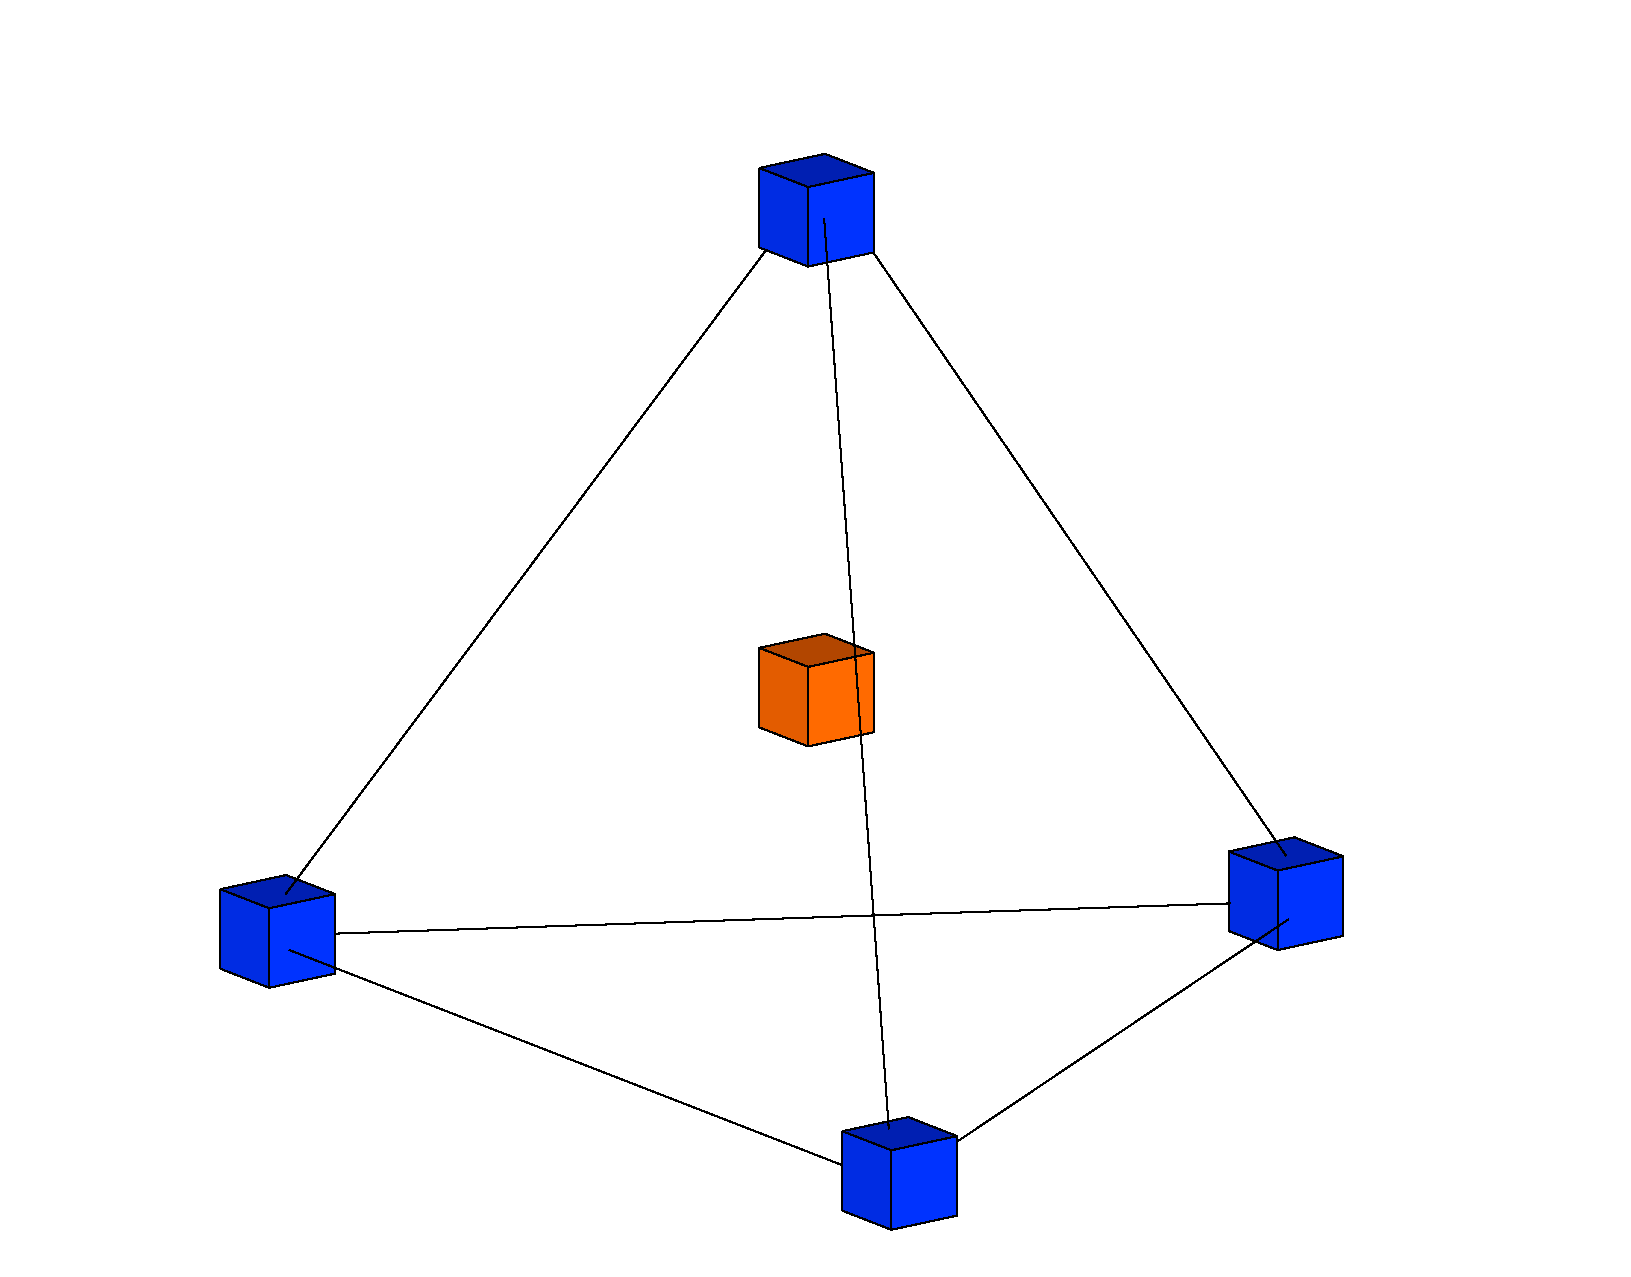
\includegraphics[width=50mm]{hw03q04model.eps}
	\caption{Example layout for $k=5$ break point for Perceptron Model in $\R^3$}
	\label{breakpointR3}
	\end{figure}
	
\newpage
\item B: i, ii, v\\
Formulae i and v were seen in lecture as valid growth functions. Formula ii is similar to i, with only a combinatorial addition which is acceptable.

Formulae iii and iv make use of the floor function, $\lfloor \cdot \rfloor$. Recall that $\text{floor}(x) = \lfloor x \rfloor$ is the largest integer not greater than $x$. For both iii and iv, for low values of $N$, the results are equal to 1, which is too low to allow a dichotomy on 1 or more points.

\item C: 5\\
Solve by drawing several points and looking for a configuration that can't be properly enclosed by either interval. See Figure \ref{breakpoint2intervals}.
	\begin{figure}[ht!]
	\centering
	\includegraphics[width=50mm]{hw03q06.pdf}
	\caption{Example layout for $k=5$ break point for ``2-intervals" learning model. Due to the arrangement of the 5 points, the point on the far right cannot be enclosed within an interval, thus breaking the hypothesis set.}
	\label{breakpoint2intervals}
	\end{figure}

\item C: \(\left( 
\begin{array}{c} N+1\\ 4 \end{array}\right) + \left( \begin{array}{c} N+1\\ 2 \end{array}\right) + 1\)

Review from lecture 5 how one interval was treated: \[\left( \begin{array}{c}N+1\\2 \end{array}\right)\]
This is a combinatoric, stating ``from $N+1$ choose 2 items". The above combinatoric was then substituted into $N+1$:
\[ \left( \begin{array}{c} N+1\\ 2 \end{array}\right) + 1\]

For a ``2-intervals" learning model, there are thus 4 sections from which to choose out of $N+1$ total sections of a line containing $N$ points. One might suppose that the solution to this exercise to be  \(\left( \begin{array}{c}N+1\\4 \end{array}\right)+1\), but this does not account for the combinations that occur when the pair of intervals overlap, effectively acting like a single interval. Thus, we must add the disjoint combinations to arrive at 
\[\left( 
\begin{array}{c} N+1\\ 4 \end{array}\right) + \left( \begin{array}{c} N+1\\ 2 \end{array}\right) + 1\]

\item D: $2M+1$\\
Establish a pattern based on what we have seen so far: 
	\begin{itemize}
	\item ``1-interval" learning model with breakpoint $k=3$.
	\item ``2-interval" learning model with breakpoint $k=5$.
	\item \dots (determine the breakpoints for several more intervals)
	\item ``$M$-interval" learning model with breakpoint $k=2M+1$.
	\end{itemize}

\item D: 7\\
To approach this problem, start by drawing points, e.g. 7 points, on a circle. Next, paint the points in alternating colors. There will happen to be two adjacent points that will be the same color. Draw a triangle dissecting the circle, enclosing all points of the same color. Repeat this procedure with 8 points to see that it is not possible to shatter the points. Thus, we have determined the breakpoint $k=8$ and the maximum points that can be shattered is $N=7$. As seen in lecture, arranging points along a circle is useful for convex shapes.
See Figure \ref{trianglemaxshatter}. If $N\geq8$, it is not possible to shatter the points for this learning model.
	\begin{figure}[ht!]
	\centering
	\includegraphics[width=50mm]{hw03q09.pdf}
	\caption{$N=7$ (depicted as points on a heptagon) is the maximum number of points that can be shattered by the ``triangle" learning model.}
	\label{trianglemaxshatter}
	\end{figure}
	
\newpage
\item B. \(\left( \begin{array}{c}N+1\\2\end{array}\right)+1\)\\
Given the symmetry of the concentric circles, we can simply extend a line from the center outward. Along the radial line are placed points of alternating color. As depicted in Figure \ref{conccircle}, the ``concentric circle" learning model is similar to the ``1-interval" linear model we saw in lecture 5. The growth functions are identical: \[m_\mathcal{H}(N)=\left( \begin{array}{c}N+1\\2 \end{array}\right)+1\]
	\begin{figure}[ht!]
	\centering
	\includegraphics[width=90mm]{hw03q10.pdf}
	\caption{Extending a radial line across the concentric circles shows the similarity of the ``concentric circle" learning model to the ``1-interval" learning model.}
	\label{conccircle}
	\end{figure}
\end{enumerate}

\label{LastPage}
\end{document}